\begin{figure}[H]
  \centering
  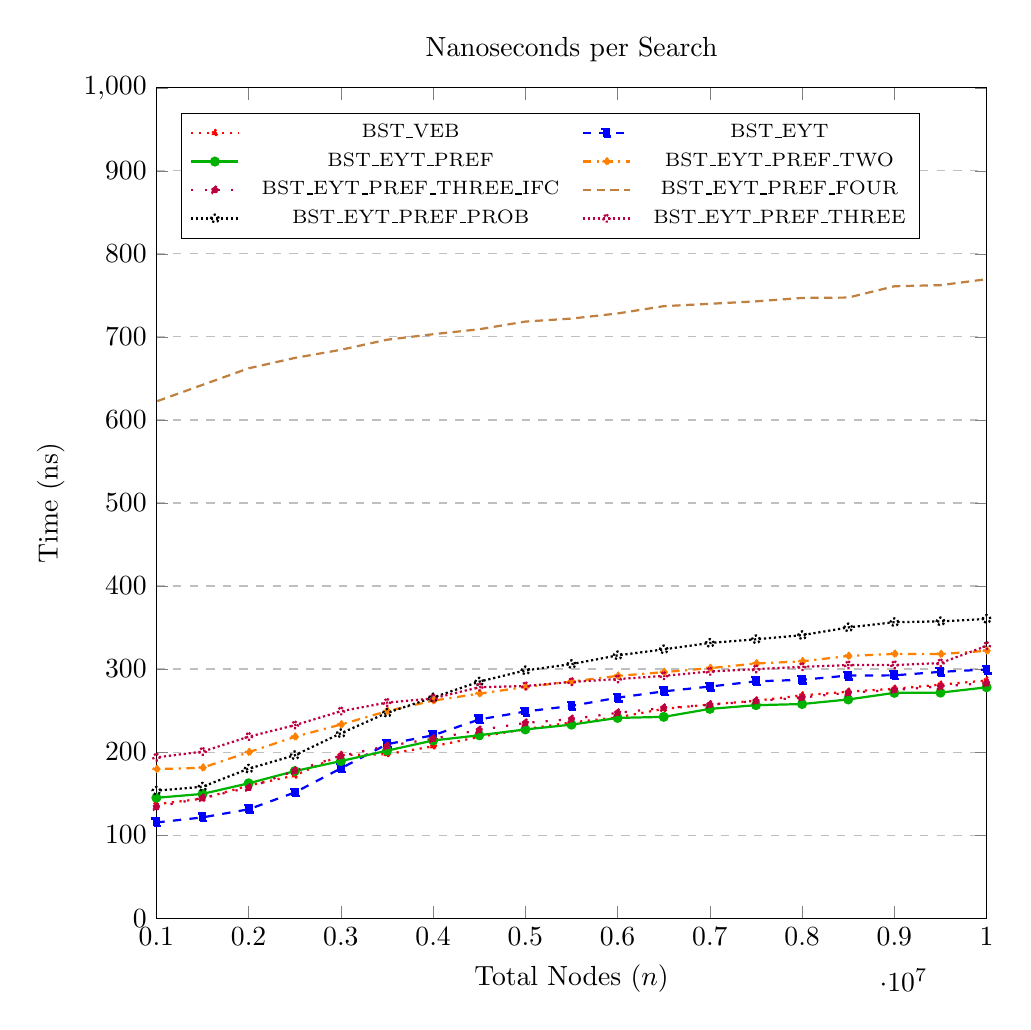
\begin{tikzpicture}
    \begin{axis}[
        title={Nanoseconds per Search},
        xlabel={Total Nodes ($n$)},
        ylabel={Time (ns)},
        width=\textwidth,
        height=1\textwidth,
        xmin=1000000, xmax=10000000,
        ymin=0, ymax=1000,
        ymajorgrids,
        grid style=dashed,
        legend columns=2,
        legend pos=north west,
        legend style={font=\scriptsize, column sep=6pt},
    ]

\addplot+[red, thick, dotted, mark=triangle*, mark options={scale=.7,fill=red}]
  coordinates {
    (500000,102.726)
    (1000000,137.13)
    (1500000,143.886)
    (2000000,159.617)
    (2500000,171.777)
    (3000000,196.365)
    (3500000,197.443)
    (4000000,206.864)
    (4500000,218.247)
    (5000000,227.587)
    (5500000,235.689)
    (6000000,241.807)
    (6500000,252.008)
    (7000000,257.294)
    (7500000,261.835)
    (8000000,268.192)
    (8500000,272.709)
    (9000000,276.222)
    (9500000,281.141)
    (10000000,286.22)
  };
\addlegendentry{BST\_VEB}

\addplot+[blue, thick, dashed, mark=square*, mark options={scale=.7,fill=blue}]
  coordinates {
    (500000,92.675)
    (1000000,115.188)
    (1500000,121.277)
    (2000000,131.068)
    (2500000,151.288)
    (3000000,180.365)
    (3500000,209.468)
    (4000000,220.168)
    (4500000,239.277)
    (5000000,248.806)
    (5500000,255.591)
    (6000000,265.492)
    (6500000,273.073)
    (7000000,278.9)
    (7500000,285.153)
    (8000000,287.066)
    (8500000,292.138)
    (9000000,292.386)
    (9500000,296.622)
    (10000000,299.403)
  };
\addlegendentry{BST\_EYT}

\addplot+[green!70!black, thick, solid, mark=*, mark options={scale=.7,fill=green!70!black}]
  coordinates {
    (500000,114.144)
    (1000000,144.896)
    (1500000,149.584)
    (2000000,162.358)
    (2500000,177.057)
    (3000000,189.114)
    (3500000,201.675)
    (4000000,213.915)
    (4500000,220.231)
    (5000000,227.221)
    (5500000,233.019)
    (6000000,241.118)
    (6500000,242.36)
    (7000000,252.003)
    (7500000,256.477)
    (8000000,257.834)
    (8500000,263.357)
    (9000000,271.258)
    (9500000,271.583)
    (10000000,278.004)
  };
\addlegendentry{BST\_EYT\_PREF}

\addplot+[orange, thick, dashdotted, mark=diamond*, mark options={scale=.7,fill=orange}]
  coordinates {
    (500000,140.616)
    (1000000,179.446)
    (1500000,181.092)
    (2000000,199.792)
    (2500000,218.321)
    (3000000,233.176)
    (3500000,249.186)
    (4000000,261.884)
    (4500000,270.372)
    (5000000,278.299)
    (5500000,284.965)
    (6000000,291.716)
    (6500000,296.259)
    (7000000,301.062)
    (7500000,306.649)
    (8000000,309.25)
    (8500000,315.71)
    (9000000,318.235)
    (9500000,317.96)
    (10000000,321.966)
  };
\addlegendentry{BST\_EYT\_PREF\_TWO}

\addplot+[purple, thick, loosely dotted, mark=pentagon*, mark options={scale=.7,fill=purple}]
  coordinates {
    (500000,104.743)
    (1000000,133.899)
    (1500000,144.771)
    (2000000,157.02)
    (2500000,177.389)
    (3000000,195.294)
    (3500000,207.233)
    (4000000,215.992)
    (4500000,226.521)
    (5000000,235.098)
    (5500000,239.645)
    (6000000,247.259)
    (6500000,253.145)
    (7000000,256.917)
    (7500000,261.485)
    (8000000,265.658)
    (8500000,271.4)
    (9000000,274.776)
    (9500000,279.107)
    (10000000,282.98)
  };
\addlegendentry{BST\_EYT\_PREF\_THREE\_IFC}

\addplot+[brown, thick, densely dashed, mark=x*, mark options={scale=.7,fill=brown}]
  coordinates {
    (500000,520.997)
    (1000000,622.281)
    (1500000,642.272)
    (2000000,662.231)
    (2500000,674.684)
    (3000000,684.506)
    (3500000,696.65)
    (4000000,703.277)
    (4500000,709.252)
    (5000000,718.52)
    (5500000,722.122)
    (6000000,728.272)
    (6500000,737.057)
    (7000000,739.914)
    (7500000,742.858)
    (8000000,746.992)
    (8500000,747.414)
    (9000000,761.055)
    (9500000,762.346)
    (10000000,769.524)
  };
\addlegendentry{BST\_EYT\_PREF\_FOUR}

\addplot+[black, thick, densely dotted, mark=o, mark options={scale=.7,fill=black}]
  coordinates {
    (500000,147.275)
    (1000000,153.474)
    (1500000,158.197)
    (2000000,179.932)
    (2500000,196.111)
    (3000000,222.617)
    (3500000,247.246)
    (4000000,265.668)
    (4500000,284.784)
    (5000000,298.337)
    (5500000,305.913)
    (6000000,316.443)
    (6500000,323.66)
    (7000000,331.411)
    (7500000,335.81)
    (8000000,340.752)
    (8500000,350.089)
    (9000000,356.393)
    (9500000,357.411)
    (10000000,360.339)
  };
\addlegendentry{BST\_EYT\_PREF\_PROB}

\addplot+[purple, thick, densely dotted, mark=pentagon, mark options={scale=.7,fill=purple}]
  coordinates {
    (500000,181.189)
    (1000000,193.529)
    (1500000,200.55)
    (2000000,218.474)
    (2500000,232.343)
    (3000000,249.176)
    (3500000,259.572)
    (4000000,264.605)
    (4500000,278.065)
    (5000000,279.55)
    (5500000,284.455)
    (6000000,287.871)
    (6500000,291.725)
    (7000000,297.017)
    (7500000,299.824)
    (8000000,302.665)
    (8500000,304.736)
    (9000000,304.825)
    (9500000,307.16)
    (10000000,327.856)
  };
\addlegendentry{BST\_EYT\_PREF\_THREE}
    \end{axis}
  \end{tikzpicture}
  \caption[Average Nanoseconds per Search of different Implementations]{Average Nanoseconds per Search (\texttt{contains()}) for the different implementations. We do not take into account the time take to build the respective trees and we always run $q=1000000$ lookups.}
  \label{fig:nspsearch}
\end{figure}
